% This must be in the first 5 lines to tell arXiv to use pdfLaTeX, which is strongly recommended.
\pdfoutput=1
% In particular, the hyperref package requires pdfLaTeX in order to break URLs across lines.

\documentclass[11pt]{article}

% Change "review" to "final" to generate the final (sometimes called camera-ready) version.
% Change to "preprint" to generate a non-anonymous version with page numbers.
\usepackage[final]{acl}

% Standard package includes
\usepackage{times}
\usepackage{latexsym}

% For proper rendering and hyphenation of words containing Latin characters (including in bib files)
\usepackage[T1]{fontenc}
% For Vietnamese characters
% \usepackage[T5]{fontenc}
% See https://www.latex-project.org/help/documentation/encguide.pdf for other character sets

% This assumes your files are encoded as UTF8
\usepackage[utf8]{inputenc}

% This is not strictly necessary, and may be commented out,
% but it will improve the layout of the manuscript,
% and will typically save some space.
\usepackage{microtype}

% This is also not strictly necessary, and may be commented out.
% However, it will improve the aesthetics of text in
% the typewriter font.
\usepackage{inconsolata}

%Including images in your LaTeX document requires adding
%additional package(s)
\usepackage{graphicx}
\usepackage{subcaption}

\usepackage{acronym}
\usepackage[inline]{enumitem}
\usepackage{booktabs}
\usepackage{tabularx}
% MUST BE THE LAST IMPORT
\usepackage{cleveref}

\acrodef{acti}[ACTI]{Automatic Conspiracy Theory Identification}
\acrodef{llm}[LLM]{Large Language Model}

\newcommand{\meta}[1]{{\color{blue}#1}}

% If the title and author information does not fit in the area allocated, uncomment the following
%
%\setlength\titlebox{<dim>}
%
% and set <dim> to something 5cm or larger.

\title{Large Language Models Project \\
Bertinoro International Spring School (BISS) 2024}

% Author information can be set in various styles:
% For several authors from the same institution:
% \author{Martina Baiardi \and Davide Domini \and Nicolas Farabegoli \and Alessandro Petrella \and Gianni Tumedei }
%         Address line \\ ... \\ Address line}
% if the names do not fit well on one line use
%         Author 1 \\ {\bf Author 2} \\ ... \\ {\bf Author n} \\
% For authors from different institutions:
% \author{Author 1 \\ Address line \\  ... \\ Address line
%         \And  ... \And
%         Author n \\ Address line \\ ... \\ Address line}
% To start a separate ``row'' of authors use \AND, as in
% \author{Author 1 \\ Address line \\  ... \\ Address line
%         \AND
%         Author 2 \\ Address line \\ ... \\ Address line \And
%         Author 3 \\ Address line \\ ... \\ Address line}


\author{
  Martina Baiardi \\
  University of Bologna \\
  {\bf m.baiardi@unibo.it} \\ \And
  Davide Domini \\
  University of Bologna \\
  {\bf davide.domini@unibo.it} \\  \And
  Nicolas Farabegoli \\
  University of Bologna \\
  {\bf nicolas.farabegoli@unibo.it} \\  \AND
  Alessandro Petrella\\
  University of Bologna \\
  {\bf alessandro.petrella@unibo.it} \\ \And
  Gianni Tumedei \\
  University of Bologna \\
  {\bf gianni.tumedei2@unibo.it}
}

\begin{document}

\maketitle

\begin{abstract}
Several social network platforms - such as Telegram, 4chan, and Parler - do not employ strong moderation
policies, causing the proliferation of conspiracy theories in many contexts, like COVID-19 or the war
in Ukraine, and thus diffusing dangerous ideas and generating social harm among their communities.
%
In this paper, we present the process to fine-tune two \acp{llm} architectures
on an Italian dataset from an EVALITA challenge, that requires identifying
conspiracy theories in posts coming from Telegram.
%
We provide details about the two adopted architectures, the model configuration and the training
process adopted in our experiments.
%
%\meta{Briefly summarise the finding of the experiments}
Results show that our proposed models outperform both the baseline provided by the organizers on kaggle and 
the results of the same models without fine-tuning.

\meta{ACTI-A task / ACTI task / subtask}
\end{abstract}

\section{Task description}\label{sec:task-description}
We conducted a comparative study between \emph{Encoder-based} and \emph{Decoder-based} architectures
on the same task.
%
Specifically, we worked on the \emph{\ac{acti}}~\footnote{\url{https://russogiuseppe.github.io/ACTI/}}
task, that requires identifying conspiracy theories coming from lax moderated policies platforms like
Telegram, 4chan, and Parler.
%
We focused on the \emph{Subtask A}, where a system must recognise if a Telegram post is conspiratorial
or not.
%
To be flagged as conspiratorial, a post must:
\begin{enumerate*}[label=(\roman{*})]
  \item express the belief that major events are controlled by and/or manipulated by powerful people protecting their interests; or
  \item interpret events in a way that supports conspiracy theories.
\end{enumerate*}
A sentence is considered conspiratorial even if it shares some claims intended to undermine commonly accepted views on societal issues.

\section{Dataset description}\label{sec:dataset-description}
The dataset for \ac{acti}-A is in CSV format and contains three columns, namely:
\begin{enumerate*}[label=(\roman*)]
  \item \textbf{id}: represents a unique identifier for the post;
  \item \textbf{comment\_text}: contains the raw text written in the post; and
  \item \textbf{conspiratorial}: represents a binary label where 0 indicates that the post is not conspiratorial,
    while 1 indicates conspiratorial content.
\end{enumerate*}
The dataset is split into two separate CSV files: one, meant for the training process, lists
1842 records, while the other includes 460 posts for testing purposes.
%
Notably, since the task was part of a challenge, the second dataset did not contain the
\textbf{conspiratorial} column by default.
%
Therefore, the test set was initially labelled by computing the encoding of each sentence using an auxiliary LLM,
and subsequently, a clustering algorithm was employed in the latent space.
%
However, after an analysis, we noticed that several sentences had been mislabeled.
%
Fortunately, the \ac{acti} team was kind enough to provide the
missing labels upon our request.

\section{Related Work}\label{sec:related-work}

\meta{citare gli altri lavori che sono stati fatti per il task ACTI-A}\cite{russo2023actievalita2023overview} 
\footnote{\url{https://ceur-ws.org/Vol-3473/}}

\section{Architecture overview}\label{sec:architecture-overview}
To tackle the \ac{acti}-A subtask, we explored two alternative architectures: an encoder-based one, and
a decoder-based one. Both are detailed in this section.

\subsection{Encoder}
Encoder-based classifiers, among which BERT \cite{devlin-etal-2019-bert} is the most famous one, require the
pre-processed input text to undergo a tokenization process, where each sequence of tokens gets also prepended
with a \texttt{[CLS]} token, left-padded up to the maximum sequence length, or truncated down to it if longer.
For tasks that require splitting the input in multiple parts, an additional \texttt{[SEP]} token can be used.

Processed by the hidden encoding layers, each applying self-attention and passing the result to a feed-forward
neural network, input tokens are transformed into contextual embeddings, as shown in \Cref{fig:encoder-block}. Notably, we are only interested in
the final hidden state corresponding to the \texttt{[CLS]} token, that contains an aggregate representation of
the entire input sequence, and can be fed to a linear classifier to obtain the probability distribution of the
input belonging to one of the classes.

\begin{figure}
  \centering
  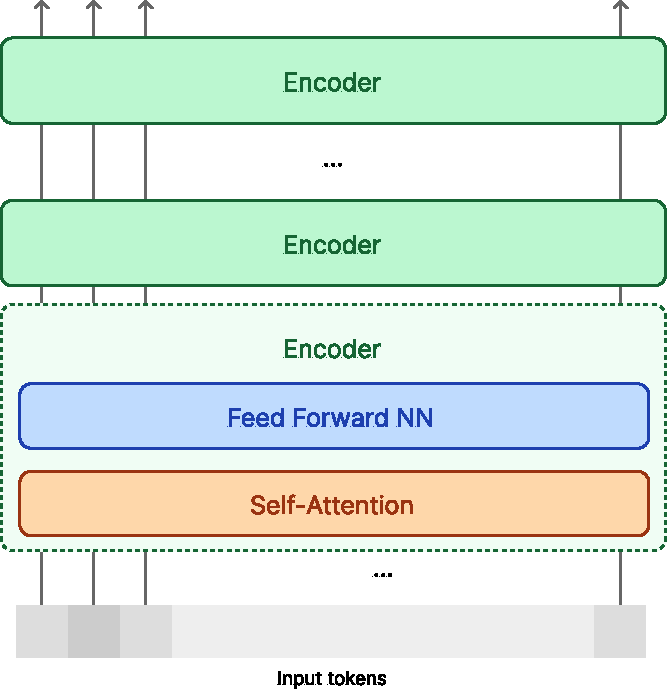
\includegraphics[width=0.8\linewidth]{figures/encoder-block.pdf}
  \caption{
    An encoder block, composed by a self-attention layer and a feed forward neural network.
  }
  \label{fig:encoder-block}
\end{figure}

\subsection{Decoder}
The decoder-based architecture we adopted is very similar to the encoder one, employing a tokenizer, followed
by the decoder model, with a classification layer on top.

For the tokenization process, the main difference when compared to the encoder solution is the absence of the \texttt{[CLS]} token. 
In fact, due to the auto-regressive nature
of decoder-only models, the last token is used to make the prediction, instead of the first.

\Cref{fig:decoder-block} shows the input passing through multiple decoder blocks, each composed by a masked 
self-attention layer and a feed-forward neural network. The masking makes it so each token only attends to previous tokens in the sequence, maintaining a unidirectional context. The final hidden state, corresponding to the last
token in the sequence, is fed to the linear layer on top of the stack of decoders. Its output dimension is equal to 
the number of labels of the given task.
%
Alternatively, and less commonly, a special token's embedding or an aggregation of all token embeddings can be
used as input for the classifier.

\begin{figure}
  \centering
  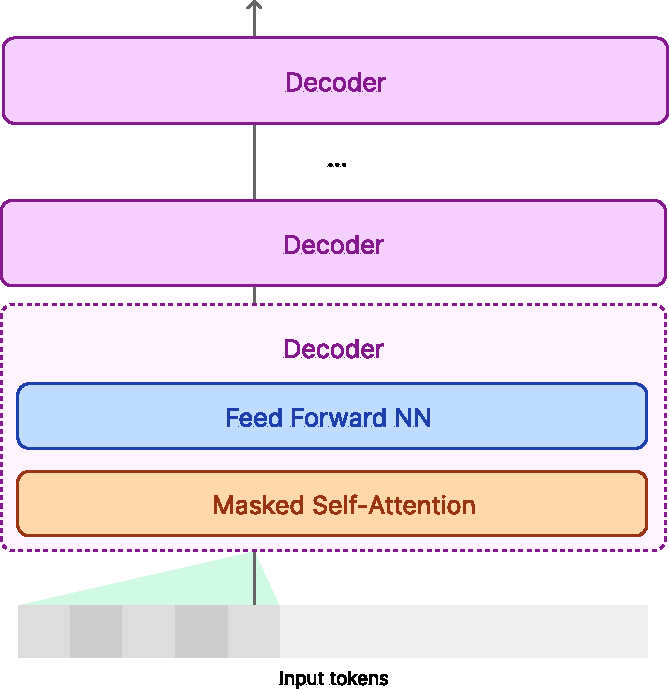
\includegraphics[width=0.8\linewidth]{figures/decoder-block.pdf}
  \caption{
    A decoder block with its masked self-attention layer and feed forward neural network.
  }
  \label{fig:decoder-block}
\end{figure}

\section{Experimental setup}\label{sec:experimental-setup}

\subsection{Preprocessing}\label{sec:preprocessing}
The preprocessing stage is a fundamental part in preparing the dataset for fine-tuning a \ac{llm}.
%
This process ensures that the data is clean, consistent, and in a format suitable for the next stages.
%
The same preprocessing procedure has been applied for both the models taken into account in \Cref{sec:model-config}.
%
In the following,
we report the steps we adopted for the preprocessing stage.

\paragraph{Dataset exploration}
We used Pandas~\cite{reback2020pandas} to build a DataFrame from the CSV dataset files,
for extracting information and data manipulation.

Preliminary,
a dataset exploration is performed to understand the categorical labels' distribution,
and the posts' length provided in the dataset.
%
\Cref{fig:class-frequency} depicts the class distribution for the \emph{training set} (left chart),
and the \emph{test set} (right chart).
%
Notably,
both the classes for the training and test set are well-balanced,
requiring no rebalancing countermeasure.

Another aspect we are interested in is the post length distribution,
since we are limited in the number of token each model can accept.
%
\Cref{fig:words-distribution} shows the distribution of the posts' length divided by training and test set.
%
The two upper charts provide the distribution on the raw post of both the dataset,
while the two lower charts describe the distribution after the cleanup step (that we will discuss in the next paragraph).
%
As can be observed,
the majority of the posts are concentrated in the range $0-500$ words,
meaning that the most of the dataset will not be truncated when input to the model.
%
The posts' cleanup process do not significantly impact the length distribution of the posts in the datasets.

\paragraph{Text cleaning}
To remove noise from the input data,
we processed the raw posts to remove any irrelevant content for the model's fine-tuning.
%
In particular,
we conducted the following operations:
\begin{enumerate*}[label=(\roman{*})]
  \item remove all the extra space;
  \item remove HTML tags and special characters like \texttt{@};
  \item remove all the http links; and
  \item remove all the \texttt{\#} but preserving the text associated to the hashtag.
\end{enumerate*}
Then,
the dataset is updated with the cleaned version of the posts,
preserving the same file structure.


\begin{figure*}
  \centering
  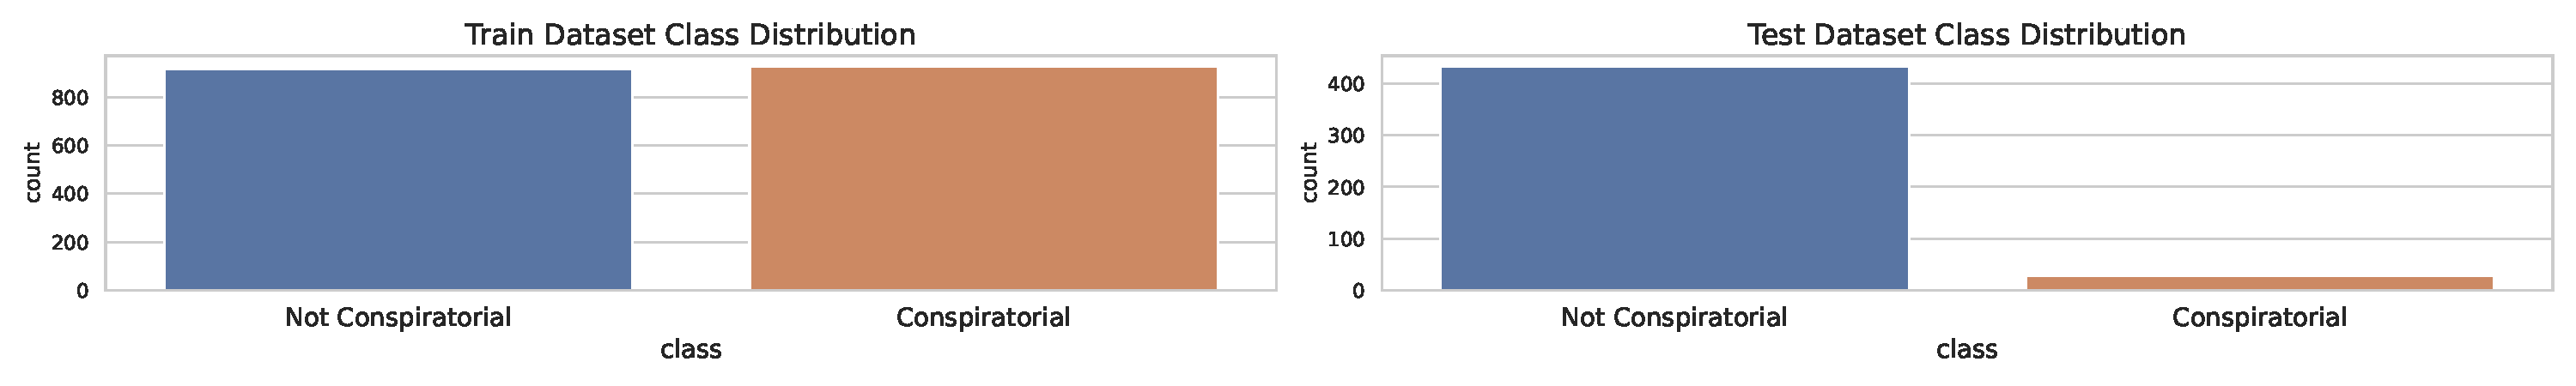
\includegraphics[width=\textwidth]{figures/class_distribution.pdf}
  \caption{
    Class distribution between the \emph{training set} and the \emph{test set}.
  }
  \label{fig:class-frequency}
\end{figure*}

\begin{figure*}
  \centering
  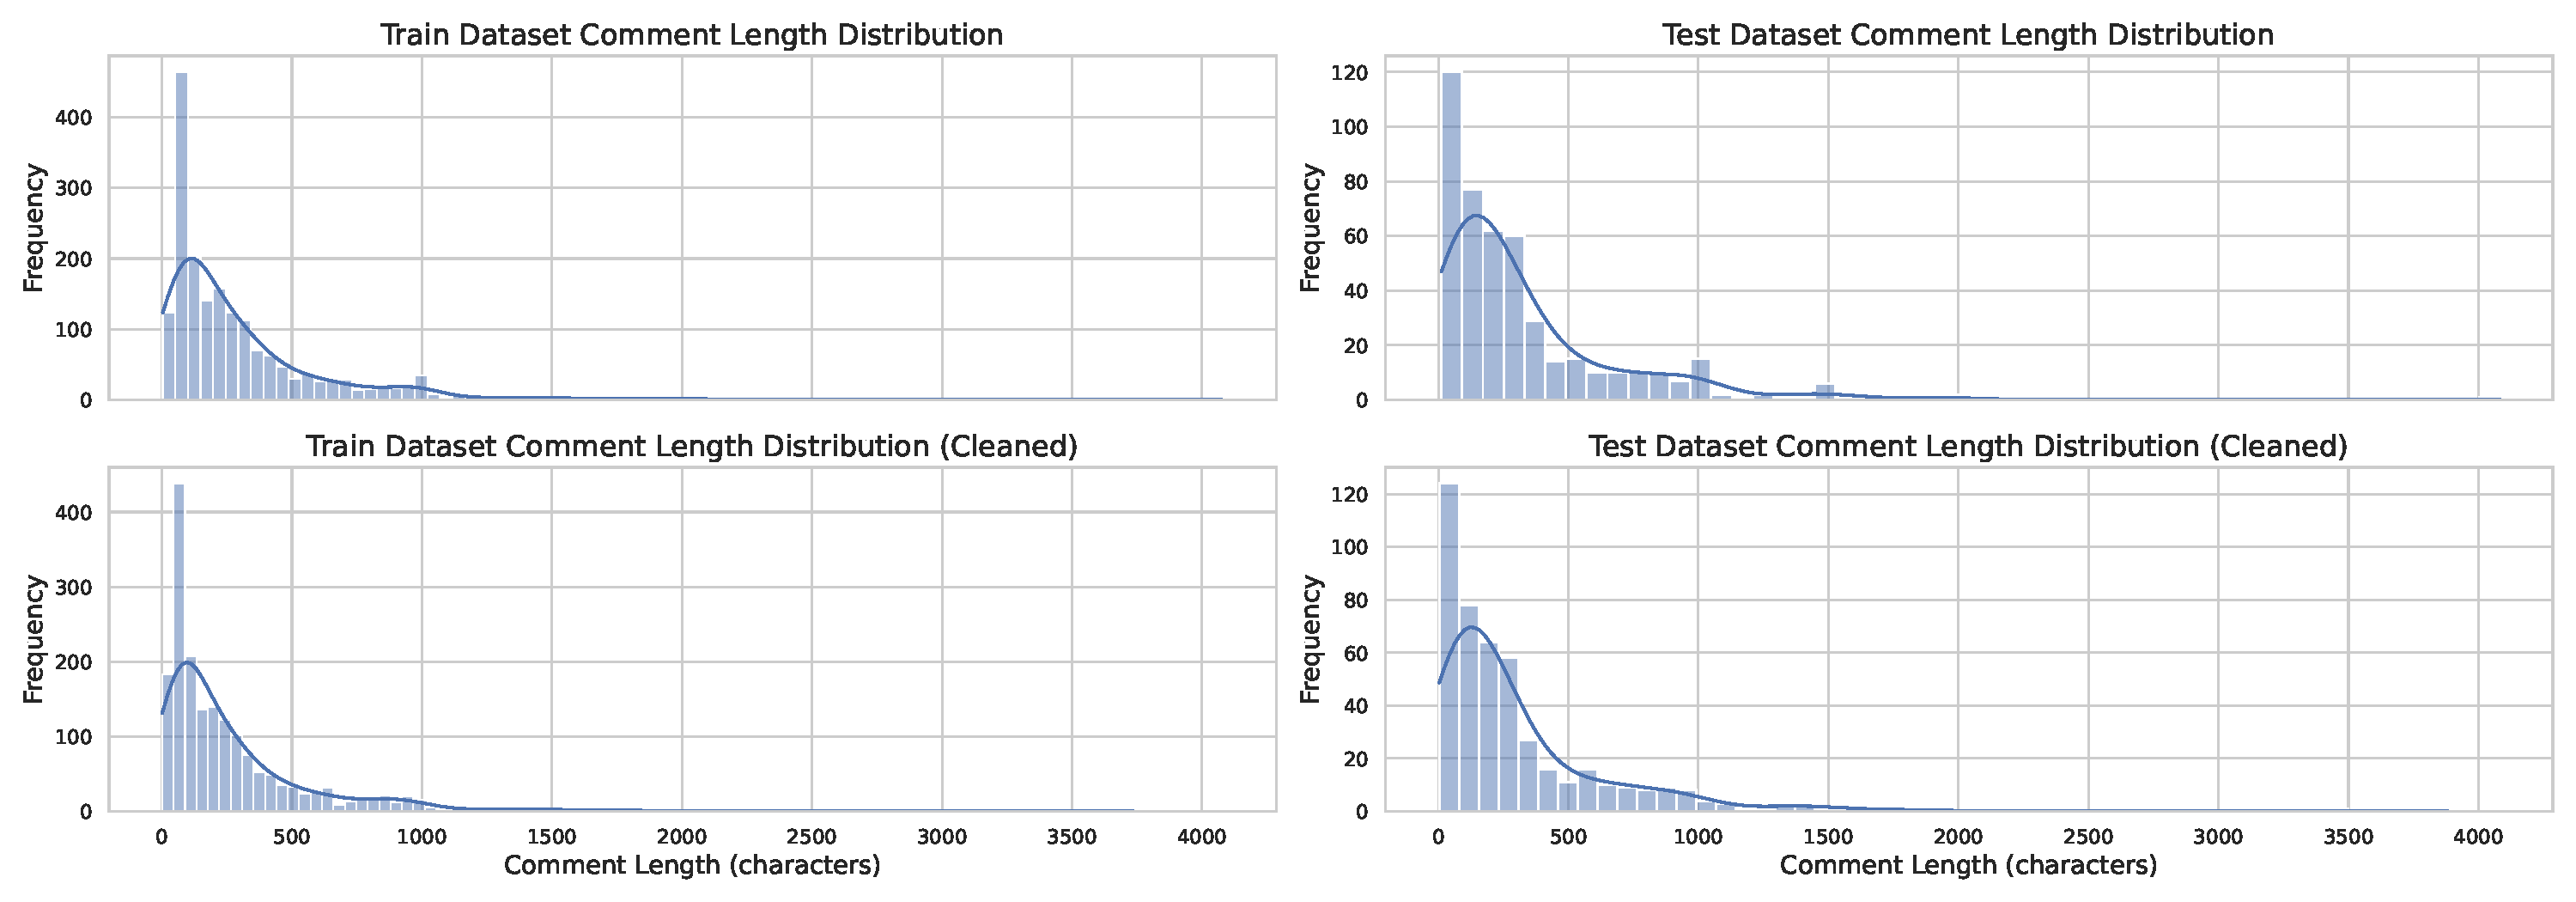
\includegraphics[width=\textwidth]{figures/comment_length_distribution.pdf}
  \caption{
    Comment length distribution for both the training dataset (on the left) and test dataset
    (on the right).
    %
    The upper charts refer to the raw content of posts, coming from the original dataset;
    in the lower charts, our cleanup preprocessing has been applied to the content.
  }
  \label{fig:words-distribution}
\end{figure*}

\subsection{Model configuration}\label{sec:model-config}
While solving ACTI-A subtask, we also compared performances of two different Transformer-based architectures,
the first one based on an \emph{Encoder} neural network, and the second one on a \emph{Decoder} neural network.

\paragraph{Encoder}

We adopted a RoBERTa-based Language Model named \texttt{UmBERTo Commoncrawl Cased},
which is trained on the large italian subcorpus of \texttt{OSCAR project} ~\footnote{\url{https://oscar-project.org/}}.
%
To address the chosen challenge, we added to this model a final layer for classification,
which returns a value for each class specified,
in our case two classes, for identifying if a text is conspiratorial or not.

Before training the model on our task we performed preprocessing, as described in \Cref{sec:preprocessing},
and then tokenization (\Cref{fig:preprocessing-and-tokenization-encoder}).
%
Concerning tokenization, \texttt{CamembertTokenizerFast} is adopted,
it normalizes strings input both regarding delimeters of the text,
but also adds a left-side padding where the input is smaller than the maximum sequence length,
that we fixed at $ 256 $ characters.
%
\begin{figure}
  \centering
  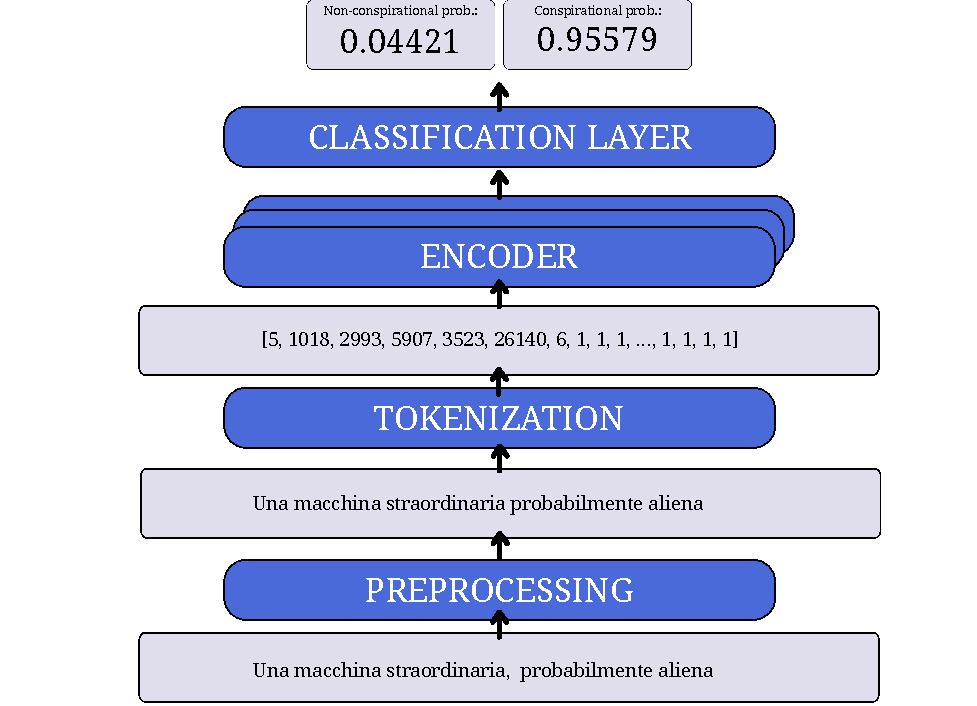
\includegraphics[width=\linewidth]{figures/encoder.pdf}
  \caption{
    Input manipulation before passing it to the encoder LLM model.
    The image exemplifies the manipulation output obtained after the cleanup process and the application of the tokenization function.
  }
  \label{fig:preprocessing-and-tokenization-encoder}
\end{figure}

\paragraph{Decoder}

The decoder model adopted to be fine-tuned is a small \texttt{OpenAI GPT2} model adapted to italian language~\cite{de-vries-nissim-2021-good}.
%
Similarly to the encoder configuration,
text is preprocessed and then tokenized before being served to the model.
%
Oppositely from the encoder,
text tokenization is performed using \texttt{GPT2Tokenizer}
and configured to add the padding on the right side of the text input (\Cref{fig:preprocessing-and-tokenization-decoder}).
%
This is made because, given the architecture of a decoder model,
the last token of the input sequence is used to make predictions about the next token that should follow the input,
this means that the last token of the input sequence contains all the information needed in the prediction.
%
\begin{figure}
  \centering
  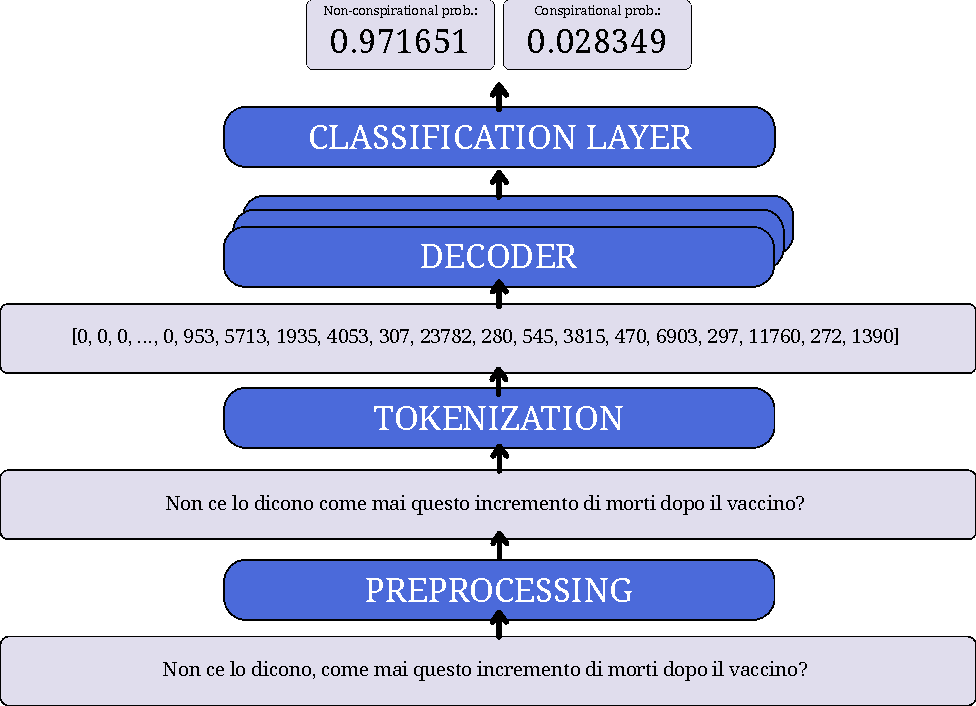
\includegraphics[width=\linewidth]{figures/decoder.pdf}
  \caption{
    Input manipulation before passing it to the decoder LLM model.
    The image exemplifies the manipulation output obtained after the cleanup process and the application of the tokenization function.
  }
  \label{fig:preprocessing-and-tokenization-decoder}
\end{figure}

\subsection{Training process}\label{sec:training-process}
During the training phase, we focused on fine-tuning two distinct models: one was encoder-only and the
  other was decoder-only (as described in~\Cref{sec:model-config}).
  We leveraged the libraries PyTorch~\cite{NEURIPS2019_9015} and HuggingFace for this process.
  To maintain consistency, we applied the same hyperparameters to both models, which included:
  \begin{enumerate*}[label=(\roman{*})]
    \item $4$ epochs of fine-tuning;
    \item a maximum sequence length of $256$; and
    \item a batch size of $16$.
  \end{enumerate*}
  \meta{TODO: Discutere delle scelte forzate dal fatto che la memoria ci ha limitato nel sequebnce length e, conseguentemente, il batch size e' stato adattato.}
  The only variation was in the learning rate, where we used $2 \cdot 10^{-5}$ for the encoder and $5 \cdot 10^{-5}$ for the decoder.
  Finally, we used the cross-entropy loss.


\section{Result and analysis}\label{sec:results-analysis}

\def\arraystretch{1.2}%
\begin{table}
  \centering
  \begin{tabularx}{\columnwidth}{X r}

    \toprule
    \textit{Model} & $F_1 score$ \\
    \midrule\midrule

    \multicolumn{2}{c}{\textbf{Baseline}} \\
    \midrule
    Kaggle Baseline & $0.5107$    \\
    EVALITA Winner &   $0.8572$  \\
    
    \midrule
    \multicolumn{2}{c}{\textbf{Proposed model with no fine-tuning}} \\
    \midrule
    
    Encoder-Only &  $0.4538$    \\
    Decoder-Only &   $0.3189$  \\
    
    \midrule
    \multicolumn{2}{c}{\textbf{Proposed model after fine-tuning}}\\
    \midrule
    
    Encoder-Only &  $0.8211$    \\
    Decoder-Only &   $0.7464$  \\
    \bottomrule
  \end{tabularx}

  \caption{\label{table:results}
    Results obtained from the models proposed, with and without fine-tuning, 
    on ACTI-A subtask. Baseline were provided by the ACTI task organizers via Kaggle.
  }
\end{table}

We evaluated the performance of our classification models using the $F_1 score$. 
Table \ref{table:results} displays the performance of our proposed model, 
along with additional scores for comparison to provide further insights into the results. 
The $F_1 scores$ were computed on the labeled test set provided by the organizers of the ACTI task.
The Kaggle baseline $F_1 scores$ is 0.5107, while the EVALITA winners achieved 0.8572. 
Our initial models, without any tuning, achieved $F_1 scores$ of 0.4538 and 0.3189 for the encoder-only 
and decoder-only configurations, respectively. After fine-tuning, the $F_1 scores$ improved to 0.8211 and 0.7464.
Comparing the results, we observe that our proposed models significantly 
outperform the baseline ($+60,77\% $ and $+46,15\%$) but do not reach the performance level of the EVALITA winners.
%
\meta{discussione sulle confusion matrix}



% \begin{figure}
%   \centering
%   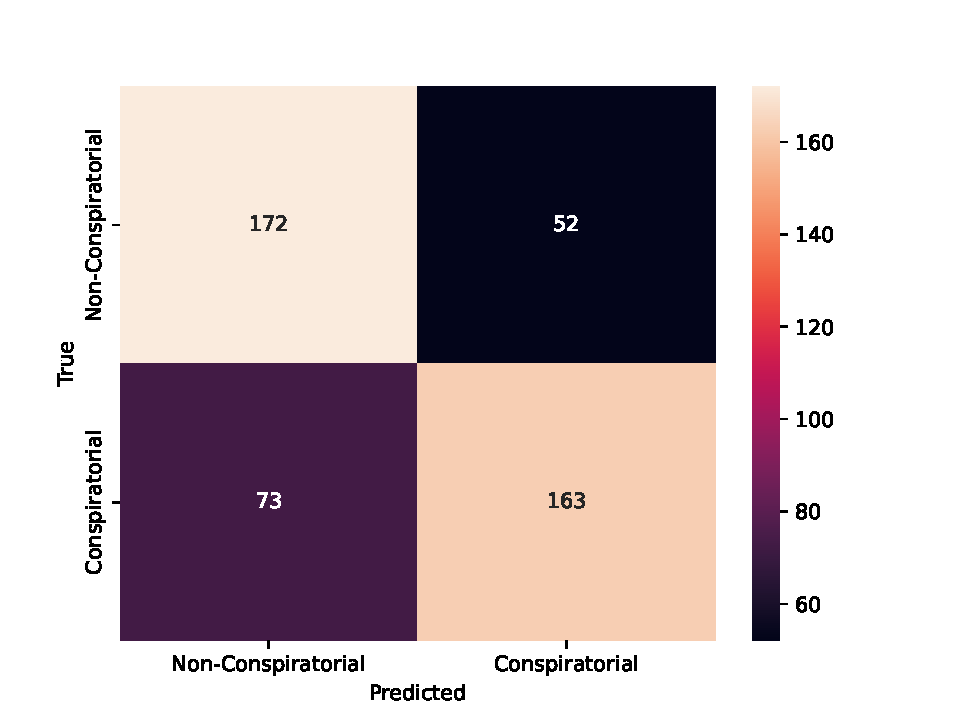
\includegraphics[width=\columnwidth]{figures/decoder-only-confusion-matrix.pdf}
%   \caption{
%    TBA}
%   \label{fig:decoder-only-cm}
% \end{figure}

% \begin{figure}
%   \centering
%   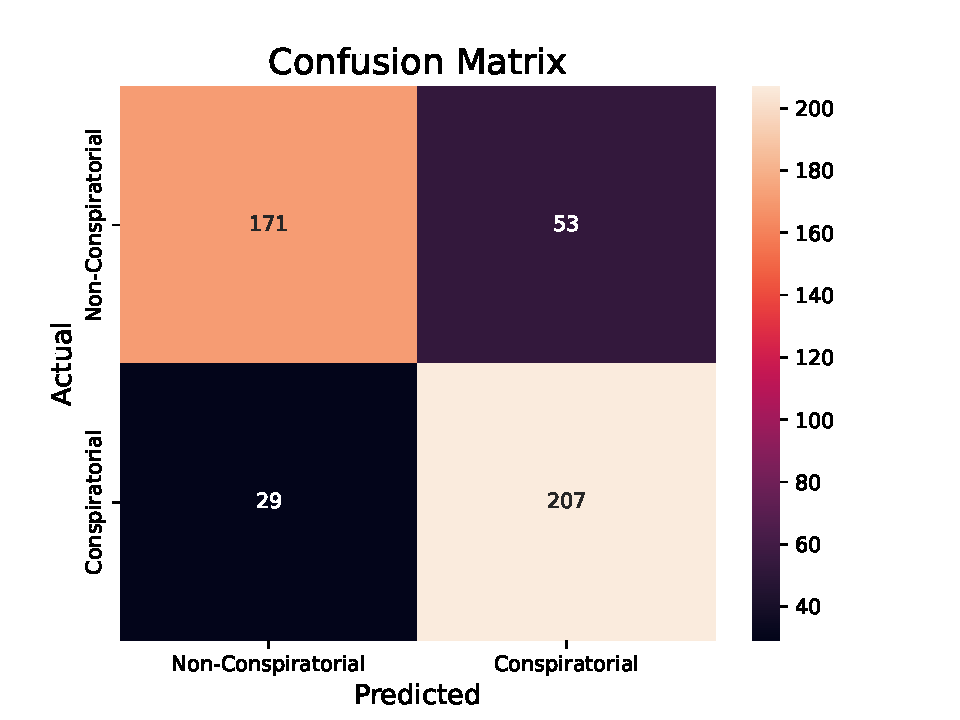
\includegraphics[width=\columnwidth]{figures/encoder-only-confusion-matrix.pdf}
%   \caption{
%    TBA}
%   \label{fig:encoder-only-cm}
% \end{figure}


\begin{figure}
    \centering
    \begin{subfigure}{\columnwidth}
        \centering
        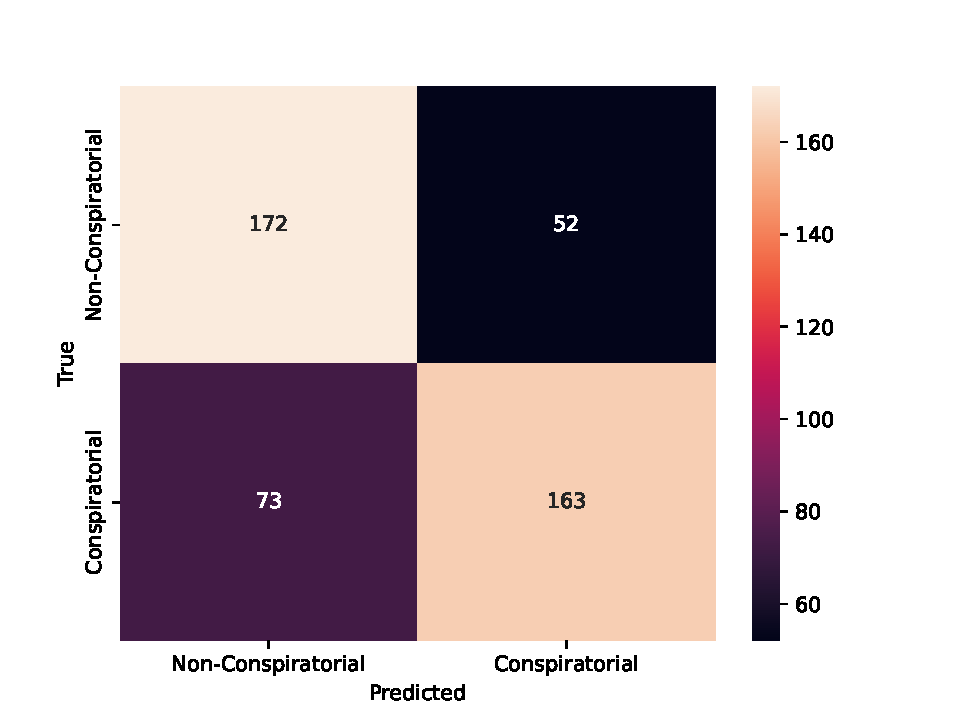
\includegraphics[width=\textwidth]{figures/decoder-only-confusion-matrix.pdf}
    \end{subfigure}
    \begin{subfigure}{\columnwidth}
        \centering
        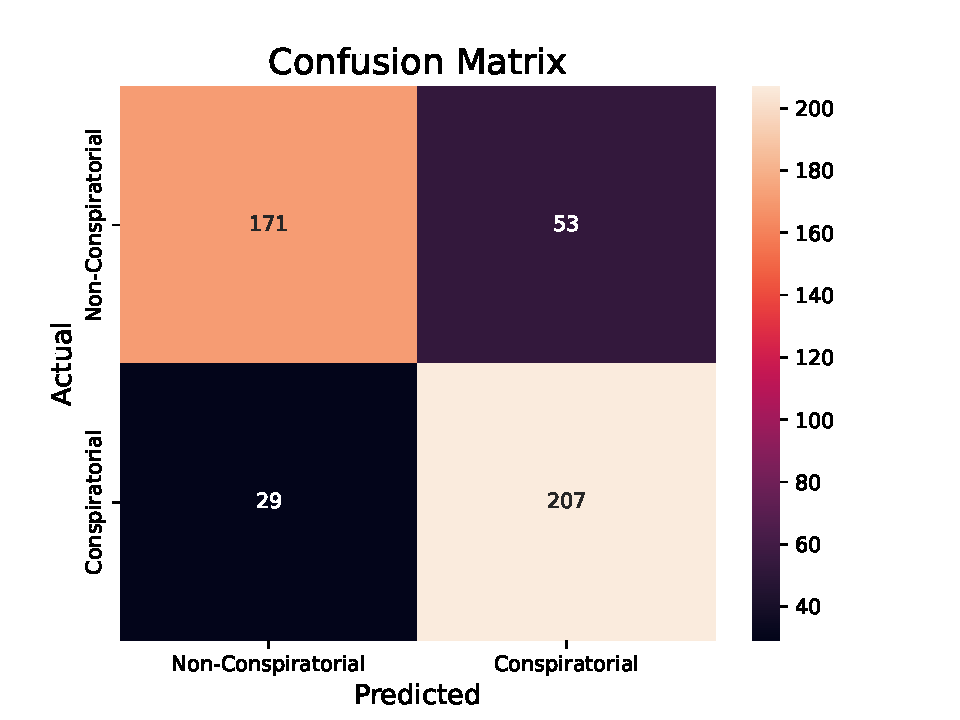
\includegraphics[width=\textwidth]{figures/encoder-only-confusion-matrix.pdf}
    \end{subfigure}
    \caption{Classification results on the test set for both encoder-only and decoder-only models.}
    \label{fig:confusion-matrix}
\end{figure}


\bibliography{bibliography}

% \appendix

% \section{Example Appendix}
% \label{sec:appendix}

% This is an appendix.

\end{document}
